\documentclass{report}
\usepackage[utf8]{inputenc} %encodage entrée
\usepackage{endnotes} %notes de fin
\usepackage{graphicx} %images
\usepackage[usenames,dvipsnames]{color} %couleurs
\usepackage{listings} %mise en forme de code source
\usepackage{xfrac}
\renewcommand\theequation{\arabic{equation}}
\usepackage{tabularx} % modifier la taille des cellules des tableaux
\usepackage{upquote}
\usepackage{textcomp}
\usepackage{pdfpages}
\usepackage[frenchb]{babel} %langue
\usepackage{amsmath} %affichage des matrices
\usepackage{lipsum} %génération de lipsum
\usepackage{verbatim} %code source
\usepackage{moreverb} %amélioration du package verbatim
\usepackage{titlesec} %formatage des chapitres
\titleformat{\chapter}[hang]{\bf\huge}{\thechapter}{2pc}{}
\usepackage[a4paper]{geometry} %mise en page
% \usepackage{varioref,amssymb,float} % polices 
% \usepackage{pgf,tikz} % permet de créer comme pstricks des figures en code LateX 
% \usetikzlibrary{calc} 
% \usepackage{pgflibraryarrows} % librairie liée à tikz 
% \usepackage{pgflibrarysnakes} 
% \usepackage{xcolor} % module de couleur pour tikz 
\geometry{hscale=0.8,vscale=0.8,centering}
%\lstinputlisting[language=Python, firstline=37, lastline=45]{source_filename.py}
\title{Algorithmes numériques -- Rapport \\ \vspace{0.5cm}Interpolation et Approximation}
\author{Axel Delsol, Pierre-Loup Pissavy}
\date{Décembre 2013}
\lstset{literate=
   {á}{{\'a}}1 {é}{{\'e}}1 {í}{{\'i}}1 {ó}{{\'o}}1 {ú}{{\'u}}1
   {Á}{{\'A}}1 {É}{{\'E}}1 {Í}{{\'I}}1 {Ó}{{\'O}}1 {Ú}{{\'U}}1
   {à}{{\`a}}1 {è}{{\`e}}1 {ì}{{\`i}}1 {ò}{{\`o}}1 {ò}{{\`u}}1
   {À}{{\`A}}1 {È}{{\`E}}1 {Ì}{{\`I}}1 {Ò}{{\`O}}1 {Ò}{{\`U}}1
   {ä}{{\"a}}1 {ë}{{\"e}}1 {ï}{{\"i}}1 {ö}{{\"o}}1 {ü}{{\"u}}1
   {Ä}{{\"A}}1 {Ë}{{\"E}}1 {Ï}{{\"I}}1 {Ö}{{\"O}}1 {Ü}{{\"U}}1
   {â}{{\^a}}1 {ê}{{\^e}}1 {î}{{\^i}}1 {ô}{{\^o}}1 {û}{{\^u}}1
   {Â}{{\^A}}1 {Ê}{{\^E}}1 {Î}{{\^I}}1 {Ô}{{\^O}}1 {Û}{{\^U}}1
   {œ}{{\oe}}1 {Œ}{{\OE}}1 {æ}{{\ae}}1 {Æ}{{\AE}}1 {ß}{{\ss}}1
   {ç}{{\c c}}1 {Ç}{{\c C}}1 {ø}{{\o}}1 {å}{{\r a}}1 {Å}{{\r A}}1
   {€}{{\EUR}}1 {£}{{\pounds}}1
}
\lstdefinestyle{customc}{
   belowcaptionskip=1\baselineskip,
   breaklines=true,
   frame=L,
   xleftmargin=\parindent,
   language=C,
   showstringspaces=false,
   basicstyle=\footnotesize\ttfamily,
   keywordstyle=\bfseries\color{ForestGreen},
   commentstyle=\itshape\color{Plum},
   identifierstyle=\color{NavyBlue},
   stringstyle=\color{Orange},
   numbers=left,
   caption=Code : \lstname,
   captionpos=b,
}
\lstset{
upquote=true,
columns=flexible,
basicstyle=\ttfamily,
}
\addto\captionsfrench{\renewcommand{\figurename}{\textsc{Graphique}}}
\addto\captionsfrench{\renewcommand{\tablename}{\textsc{Tableau}}}
\renewcommand{\thefigure}{\thesection.\arabic{figure}}
\renewcommand{\thetable}{\thesection.\arabic{table}}
\renewcommand{\lstlistingname}{\textsc{Figure}}
\lstdefinestyle{apercu}{
  xleftmargin=2cm,
  xrightmargin=2cm,
  frame=single,
  breaklines=true,
  breakatwhitespace=true,
  breakindent=5pt,
  postbreak=\space,
  captionpos=b,
  escapeinside={\%*}{*)},
  showstringspaces=false,
  caption=Apercu : \lstname,
}
\begin{document}
  \maketitle
  \tableofcontents

  \chapter{Préambule}
    \section{Structure du programme}
    Nous avons conçu un programme principal avec menus, présenté sous la forme suivante :
    \begin{lstlisting}[style=apercu, name=Menu Principal]
Menu principal : Interpolation et Approximation

Entrez n le nombre de points : 2
%*\textit{(Saisie de la série de points...)}*)

%*\textit{(Affichage du tableau correspondant...)}*)
Quelle résolution utiliser ?
1- Newton
2- Neuville
3- Régression Linéaire
4- Approximation par une fonction exponentielle
5- Approximation par une fonction "puissance"
9- Nouvelle série de points (Menu principal)
0- Quitter
Votre choix :
    \end{lstlisting}
  \chapter{Interpolation}
  	\noindent L'interpolation, en analyse numérique, est un ensemble de méthode permettant d'obtenir une équation mathématique passant par tous les points d'une liste données.
  	\newline
  	Pour cette partie, les équations mathématiques recherchées sont des polynômes.
  	\newline
  	
  	\underline{Notation pour la suite :}
  	\vspace{0.1 cm}
  	\begin{itemize}
  	\item{La liste comporte $N$ éléments $(x_{i},y_{i})$.}
  	\item{Les polynômes recherchés sont de la forme $P_{N-1}(x)= \sum_{i=0}^{N-1} a_{i} \cdot x^{i}$.}
  	\end{itemize}
    \section{Méthode de Newton}
      \subsection{Présentation}
	    \noindent	La forme du polynôme par la méthode de Newton est la suivante : 
    	
    	$P_{N-1}(x)= \sum_{i=0}^{N-1} \left( a_{i} \cdot \prod_{j=1}^{j=i} (x-x_{j}) \right)$ \\
    		Pour se faire , on utilise une méthode de recherche de coefficients récursive appelée la méthode des \textit{différences divisées}. Le calcul des valeurs des différences divisées se fait à l'aide d'une fonction : 
    	
    	La différence divisée de degré $0$ est :
    	
    	
    	 $\forall i=1,\ldots, N :  \boldsymbol{\bigtriangledown}^{0}y_{i} = y_{i} $
    	 
    	 La différence divisée de degré $k$ est : 
    	 
    	 $\forall i=k+1,\ldots,N : \boldsymbol{\bigtriangledown}^{k}y_{i} = \frac{\bigtriangledown^{k-1}y_{i}-\bigtriangledown^{k-1}y_{k}}{x_{i}-x{k}}$
    	 \newline
    	 Ensuite, on a directement les coefficients du polynôme de Newton par la relation 
    	 
    	 $\forall i=1,\ldots,N-1 : a_{i} = \boldsymbol{\bigtriangledown}^{i}y_{(i+1)}$
    	 \newline
    	 
    	\noindent Enfin, on peut retrouver la forme développée du polynôme à l'aide de la relation :
    	 
    	 $\forall i=0,\ldots,N : P_{i}(x) = \left\{
  \begin{array}{l l}
    a_{N-1} & \quad \text{si $i$=0}\\
    a_{N-1-i} + (x-x_{N-i}) \cdot P_{i-1}(x) & \quad \text{sinon}
  \end{array} \right. $
      \subsection{Programme}
	\lstinputlisting[style=customc]{newton.c}
    \newpage
    \section{Méthode de Neuville}
      \subsection{Présentation}
	
      \subsection{Programme}
	\lstinputlisting[style=customc]{neuville.c}
    \newpage
    \section{Résultats de tests}
      \subsection{Exemple tiré d'un TD}
	\begin{table}[h]
	  \centering
	  \begin{tabular}{| c | c | c | c | c |}
	  \hline 
	  $x_{i}$ & $1$ & $2$ & $3$ & $4$ \\ 
	  \hline 
	  $y_{i}$ & $0$ & $0$ & $0$ & $6$ \\ 
	  \hline 
	  \end{tabular}
	  \caption{Série 1}
	  \label{inter_td3_ex3}
	\end{table}
	
	On obtient alors :\\ \\
	\textbf{Méthode de Newton :}\\
	$P(x)= -6.00 + 11.00 \cdot x- 6.00 \cdot x^{2}  + 1.00 \cdot x^{3} $\\
	Erreur : $0$
	\newline
	\newline
	\textbf{Méthode de Neuville :}\\
	$P(x)= -6.00 + 11.00 \cdot x- 6.00 \cdot x^{2}  + 1.00 \cdot x^{3} $\\
	Erreur : $0$
	\newline
	\newline
	
	\begin{figure}[h]
	  \centering
	  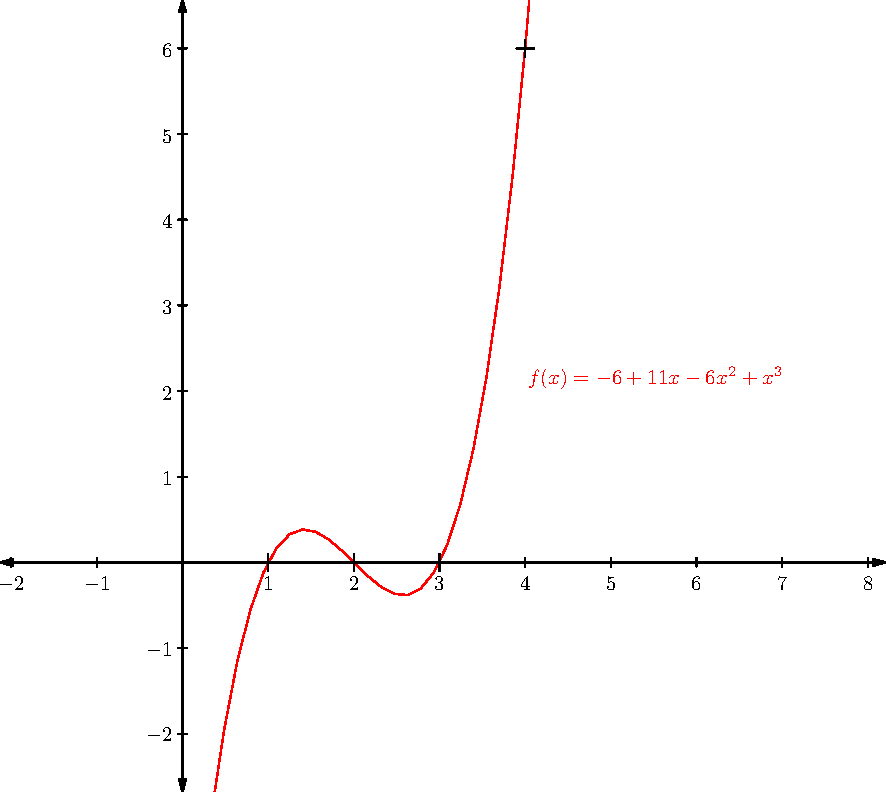
\includegraphics[scale=0.7]{graphiques/pdf_output/inter_test1.pdf}
	  \caption{Interpolations de Newton et Neuville -- (Tableau \ref{inter_td3_ex3})}
	\end{figure}
      \newpage
      
      \subsection{Densité de l'eau en fonction de la température}      
	\begin{table}[h]
	  \centering
	  \begin{tabular}{| c | c | c | c | c | c | c | c | c | c | c |}
	    \hline 
	    $x_{i}$ & $0$ & $2$ & $4$ & $6$ & $8$ & $10$ & $12$ & $14$ & $16$ & $18$ \\
	    \hline 
	    $y_{i}$ & $0.999870$ & $0.999970$ & $1.000000$ & $0.999970$ & $0.999880$ & $0.999730$ & $0.999530$ & $0.999530$ & $0.998970$ & $0.998460$ \\ 
	    \hline 
	  \end{tabular}
	  \begin{tabular}{| c | c | c | c | c | c | c | c | c | c | c |}
	    \hline
	    $x_{i}$ & $20$ & $22$ & $24$ & $26$ & $28$ & $30$ & $32$ & $34$ & $36$ & $38$ \\ 
	    \hline
	    $y_{i}$ & $0.998050$ & $0.999751$ & $0.997050$ & $0.996500$ & $0.996640$ & $0.995330$ & $0.994720$ & $0.994720$ & $0.993330$ & $0.993260$ \\
	    \hline
	  \end{tabular}
	  \caption{Mesures}
	  \label{inter_tp2_ex1_densite}
	\end{table}
	
	On obtient alors :\\ \\
	\textbf{Méthode de Newton :}\\
	$P(x) \approx 0.999870 + 7.693711 \cdot x - 13.276666 \cdot x^{2}  + 9.932303 \cdot x^{3} - 4.345460 \cdot x^{4}  + 1.259124 \cdot x^{5} - 0.258585 \cdot x^{6}  + 0.039240 \cdot x^{7} - 0.004520 \cdot x^{8}  + 0.000402 \cdot x^{9} - 0.000028 \cdot x^{10}  + 0.000002 \cdot x^{11} - 0.000000 \cdot x^{12}  + 0.000000 \cdot x^{13} - 0.000000 \cdot x^{14}  + 0.000000 \cdot x^{15} - 0.000000 \cdot x^{16}  + 0.000000 \cdot x^{17} - 0.000000 \cdot x^{18}  + 0.000000 \cdot x^{19} $\\
	Erreur : $0.000002166566117323$
	\newline
	\newline
	\textbf{Méthode de Neuville :}\\
	$P(x) \approx 0.999870 + 7.693711 \cdot x- 13.276666 \cdot x^{2}  + 9.932303 \cdot x^{3} - 4.345460 \cdot x^{4}  + 1.259124 \cdot x^{5} - 0.258585 \cdot x^{6}  + 0.039240 \cdot x^{7} - 0.004520 \cdot x^{8}  + 0.000402 \cdot x^{9} - 0.000028 \cdot x^{10}  + 0.000002 \cdot x^{11} - 0.000000 \cdot x^{12}  + 0.000000 \cdot x^{13} - 0.000000 \cdot x^{14}  + 0.000000 \cdot x^{15} - 0.000000 \cdot x^{16}  + 0.000000 \cdot x^{17} - 0.000000 \cdot x^{18}  + 0.000000 \cdot x^{19} $\\
	Erreur : $0.000028505775100296$
	\newline
	\newline
		  
	\begin{figure}[h]
	  \centering
	  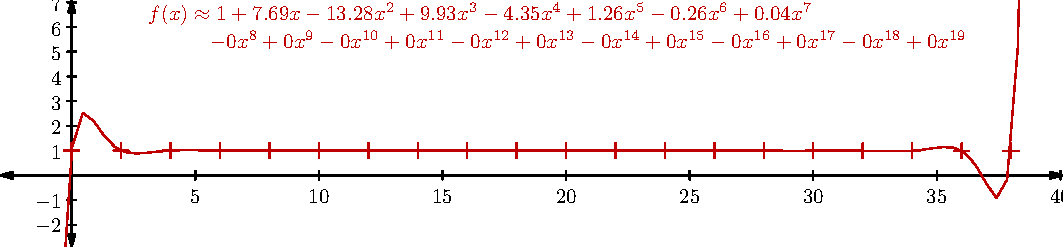
\includegraphics{graphiques/pdf_output/inter_tp2_ex1.pdf}
	  \caption{Interpolation de Newton et Neuville -- (Tableau \ref{inter_tp2_ex1_densite})}
	\end{figure}
      \newpage
    
      \subsection{3 séries}
	\begin{table}[h]
	  \centering
	  \begin{tabular}{| c | c | c | c | c | c | c | c | c | c | c | c |}
	    \hline 
	    $x_{i}$ & $10$ & $8$ & $13$ & $9$ & $11$ & $14$ & $6$ & $4$ & $12$ & $7$ & $5$ \\ 
	    \hline 
	    $y^{(1)}_{i}$ & $9.14$ & $8.14$ & $8.74$ & $8.77$ & $9.26$ & $8.10$ & $6.13$ & $3.10$ & $9.13$ & $7.26$ & $4.74$ \\ %s1
	    \hline 
	    $y^{(2)}_{i}$ & $7.46$ & $6.77$ & $12.74$ & $7.11$ & $7.81$ & $8.84$ & $6.08$ & $5.39$ & $8.15$ & $6.42$ & $5.73$ \\ %s2
	    \hline 
	    $y^{(3)}_{i}$ & $6.58$ & $5.76$ & $7.71$ & $8.84$ & $8.47$ & $7.04$ & $5.25$ & $12.50$ & $5.56$ & $7.91$ & $6.89$ \\ %s3 
	    \hline 
	  \end{tabular}	
	  \caption{Trois séries S1, S2, S3}
	  \label{inter_tp2_ex2_3series}
	\end{table}
	On obtient alors :\\ \\
	\underline{\textbf{Série 1 :}} \\ \\
	\textbf{Méthode de Newton :}\\
	$P(x) \approx -229.550000 + 299.165750 \cdot x- 173.107636 \cdot x^{2}  + 58.546955 \cdot x^{3} - 12.731862 \cdot x^{4}  + 1.859906 \cdot x^{5} - 0.184968 \cdot x^{6}  + 0.012375 \cdot x^{7} - 0.000533 \cdot x^{8}  + 0.000013 \cdot x^{9} - 0.000000 \cdot x^{10} $\\
	Erreur : $0.000000000016217532$
	\newline
	\newline
	\textbf{Méthode de Neuville :}\\
	$P(x) \approx -229.550000 + 299.165750 \cdot x- 173.107636 \cdot x^{2}  + 58.546955 \cdot x^{3} - 12.731862 \cdot x^{4}  + 1.859906 \cdot x^{5} - 0.184968 \cdot x^{6}  + 0.012375 \cdot x^{7} - 0.000533 \cdot x^{8}  + 0.000013 \cdot x^{9} - 0.000000 \cdot x^{10} $\\
	Erreur : $0.000000000012119518$
	\newline
	\newline
	\newline
	\underline{\textbf{Série 2 :}} \\ \\
	\textbf{Méthode de Newton :}\\
	$P(x) \approx -12345.190000 + 16608.066492 \cdot x- 9870.941498 \cdot x^{2}  + 3416.593892 \cdot x^{3} - 763.094009 \cdot x^{4}  + 114.979985 \cdot x^{5} - 11.842442 \cdot x^{6}  + 0.823658 \cdot x^{7} - 0.037039 \cdot x^{8}  + 0.000973 \cdot x^{9} - 0.000011 \cdot x^{10} $\\
	Erreur : $0.000000000774325735$
	\newline
	\newline
	\textbf{Méthode de Neuville :}\\
	$P(x) \approx -12345.190000 + 16608.066492 \cdot x- 9870.941498 \cdot x^{2}  + 3416.593892 \cdot x^{3} - 763.094009 \cdot x^{4}  + 114.979985 \cdot x^{5} - 11.842442 \cdot x^{6}  + 0.823658 \cdot x^{7} - 0.037039 \cdot x^{8}  + 0.000973 \cdot x^{9} - 0.000011 \cdot x^{10} $\\
	Erreur : $0.000000001033081661$
	\newline
	\newline
	\newline
	\underline{\textbf{Série 3 :}} \\ \\
	\textbf{Méthode de Newton :}\\
	$P(x) \approx -568559.640000 + 739678.381270 \cdot x- 424130.450858 \cdot x^{2}  + 141275.523224 \cdot x^{3} - 30298.693006 \cdot x^{4}  + 4375.222059 \cdot x^{5} - 431.155992 \cdot x^{6}  + 28.652640 \cdot x^{7} - 1.229803 \cdot x^{8}  + 0.030806 \cdot x^{9} - 0.000342 \cdot x^{10} $\\
	Erreur : $0.000000081067879843$
	\newline
	\newline
	\textbf{Méthode de Neuville :}\\
	$P(x) \approx -568559.640000 + 739678.381270 \cdot x- 424130.450858 \cdot x^{2}  + 141275.523224 \cdot x^{3} - 30298.693006 \cdot x^{4}  + 4375.222059 \cdot x^{5} - 431.155992 \cdot x^{6}  + 28.652640 \cdot x^{7} - 1.229803 \cdot x^{8}  + 0.030806 \cdot x^{9} - 0.000342 \cdot x^{10} $\\
	Erreur : $0.000000035876804073$
	\newpage
	\begin{figure}[h]
	  \centering
  	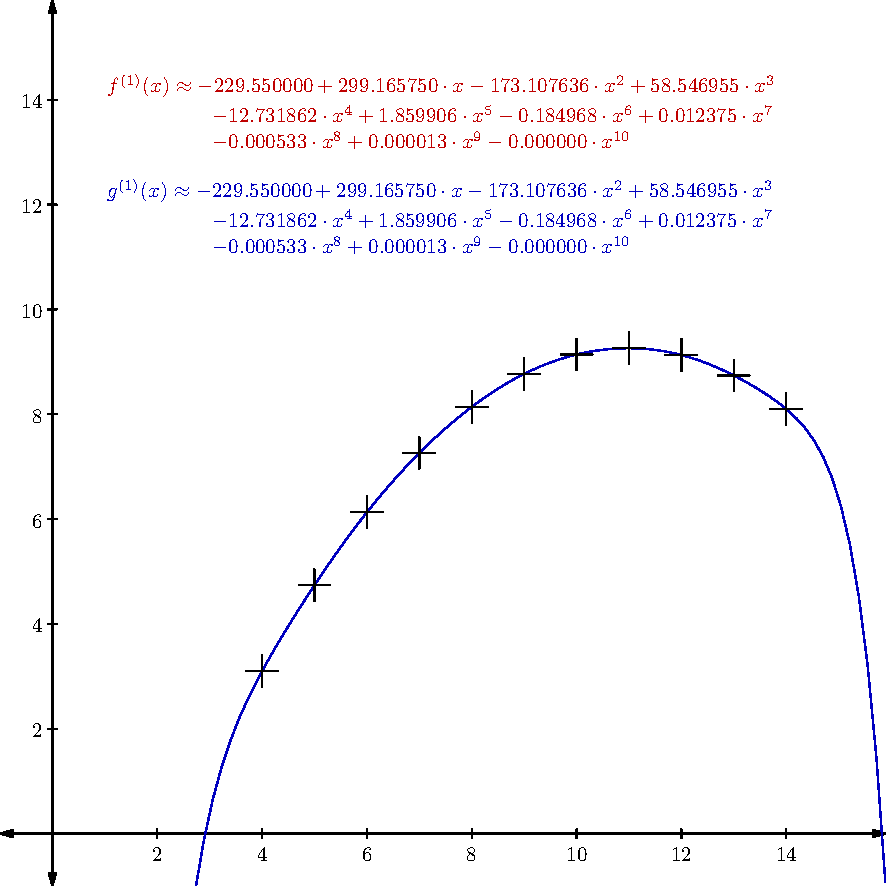
\includegraphics[scale=0.5]{graphiques/pdf_output/inter_tp2_ex2_1.pdf}
	  \caption{Interpolations de Newton et Neuville -- Série 1 (Tableau \ref{inter_tp2_ex2_3series})}
	\end{figure}
	\begin{figure}[h]
	  \centering
	  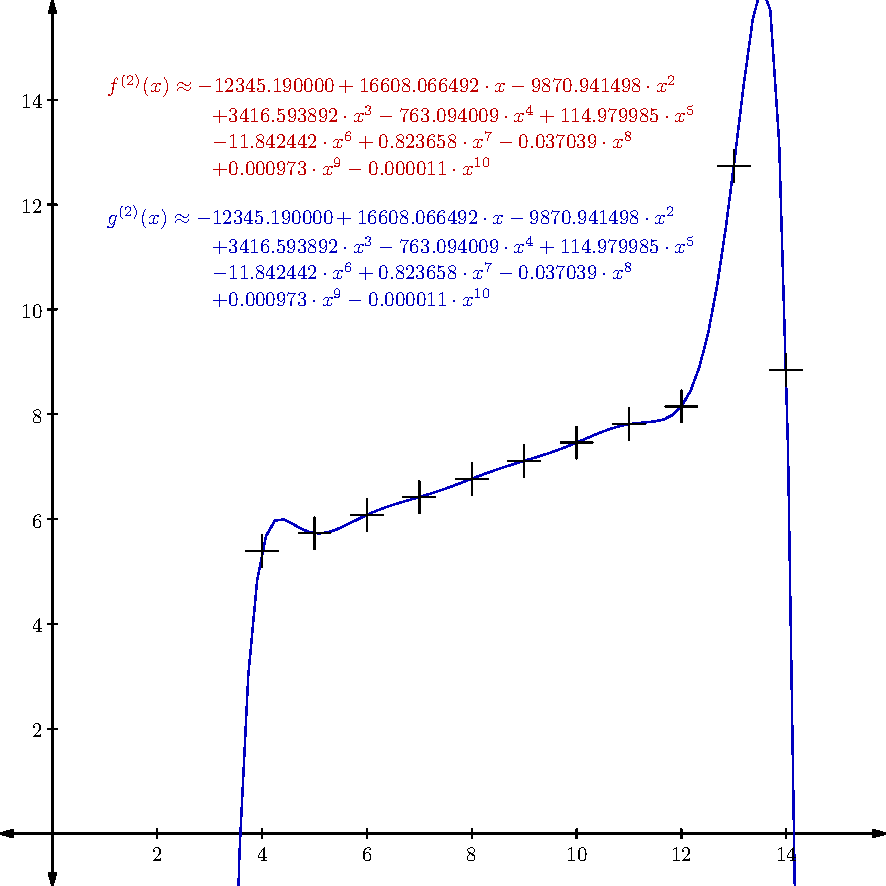
\includegraphics[scale=0.5]{graphiques/pdf_output/inter_tp2_ex2_2.pdf}
	  \caption{Interpolations de Newton et Neuville -- Série 2 (Tableau \ref{inter_tp2_ex2_3series})}
	\end{figure}
	\newpage
	\begin{figure}[h]
	  \centering
 	  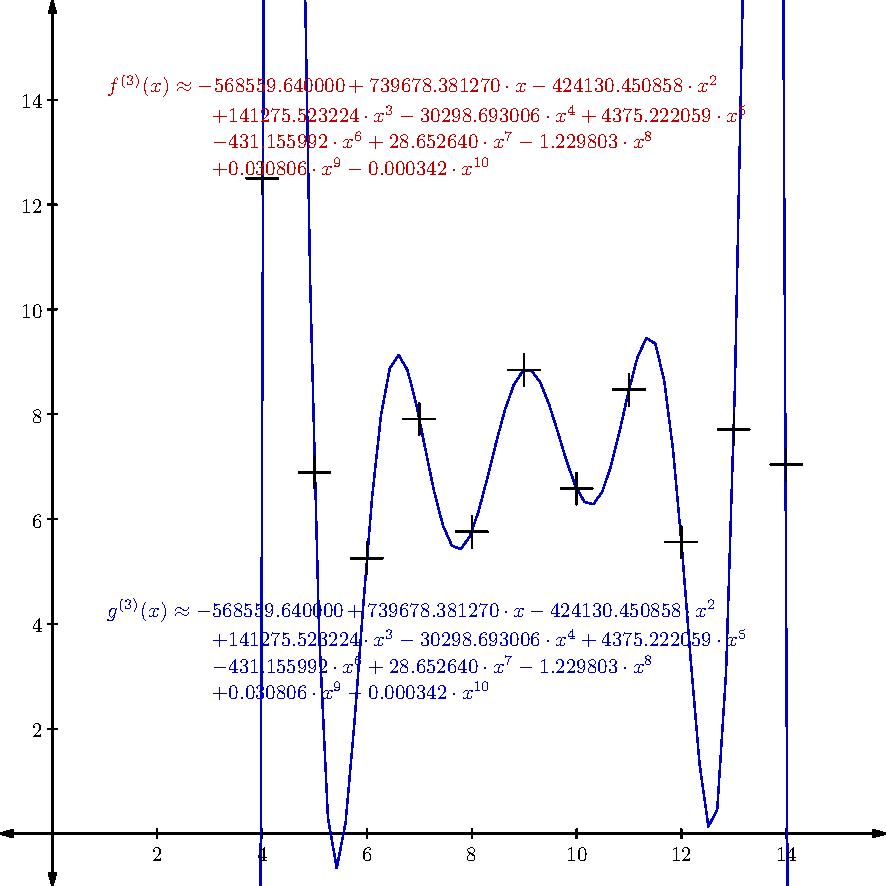
\includegraphics[scale=0.5]{graphiques/pdf_output/inter_tp2_ex2_3.pdf}
	  \caption{Interpolations de Newton et Neuville -- Série 3 (Tableau \ref{inter_tp2_ex2_3series})}
	\end{figure}
      \newpage
      \subsection{Dépenses et Revenus}
      \begin{table}[h]
% 	\centering
	\begin{tabular}{| c | c | c | c | c | c | c | c | c | c | c | c |}
	  \hline 
	  $x_{i}$ (R) & $752$ & $855$ & $871$ & $734$ & $610$ & $582$ & $921$ & $492$ & $569$ & $462$ & $907 $ \\ 
	  \hline 
	  $y_{i}$ (D) & $85$ & $83$ & $162$ & $79$ & $81$ & $83$ & $281$ & $81$ & $81$ & $80$ & $243 $ \\ 
	  \hline 
	\end{tabular}
	\newline
	\begin{tabular}{| c | c | c | c | c | c | c | c | c | c | c |}
	\hline 
	$x_{i}$ (R) & $643$ & $862$ & $524$ & $679$ & $902$ & $918$ & $828$ & $875$ & $809$ & $894$ \\ 
	\hline 
	$y_{i}$ (D) & $84$ & $84$ & $82$ & $80$ & $226$ & $260$ & $82$ & $186$ & $77$ & $223$ \\ 
	\hline 
	\end{tabular}
	\caption{Série non triée}
	\label{inter_tp2_ex3_depenses}
      \end{table}
      
      \begin{table}[h]
	\centering
	\begin{tabular}{| c | c | c | c | c | c | c | c | c | c | c | c | c | c | c |}
	  \hline 
	  $x_{i}$ (R) & $752$ & $855$ & $828$ & $734$ & $809$ & $610$ & $582$ & $492$ & $569$ & $462$ & $643$ & $862$ & $524$ & $679$ \\ 
	  \hline 
	  $y_{i}$ (D) & $85$ & $83$ & $82$ & $79$ & $77$ & $81$ & $83$ & $81$ & $81$ & $80$ & $84$ & $84$ & $82$ & $80$ \\ 
	  \hline 
	\end{tabular}
	\caption{Série triée : Partie Basse}
	\label{inter_tp2_ex3_depenses_bas}
      \end{table}
      \begin{table}[h]
	\centering
	\begin{tabular}{| c | c | c | c | c | c | c | c |}
	  \hline 
	  $x_{i}$ (R) & $902$ & $918$ & $871$ & $875$ & $921$ & $907$ & $894$ \\ 
	  \hline 
	  $y_{i}$ (D) & $226$ & $260$ & $162$ & $186$ & $281$ & $243$ & $223$ \\ 
	  \hline 
	\end{tabular}
	\caption{Série triée : Partie Haute}
	\label{inter_tp2_ex3_depenses_haut}
      \end{table}
      On obtient alors :\\ \\
      \underline{\textbf{Partie Basse :}} \\ \\
      \textbf{Méthode de Newton :}\\
	$P(x) \approx 73581192209.962601-1459287367.863513 \cdot x + 13300351.970502 \cdot x^{2} - 73765.523297 \cdot x^{3}  + 277.759281 \cdot x^{4} - 0.749863 \cdot x^{5}  + 0.001493 \cdot x^{6} - 0.000002 \cdot x^{7}  + 0.000000 \cdot x^{8} - 0.000000 \cdot x^{9}  + 0.000000 \cdot x^{10} - 0.000000 \cdot x^{11}  + 0.000000 \cdot x^{12} - 0.000000 \cdot x^{13} $\\
	Erreur : $0.018460432587224723$
	\newline
	\newline
	\textbf{Méthode de Neuville :}\\
	$P(x) \approx 73581192209.952133-1459287367.863373 \cdot x + 13300351.970501 \cdot x^{2} - 73765.523297 \cdot x^{3}  + 277.759281 \cdot x^{4} - 0.749863 \cdot x^{5}  + 0.001493 \cdot x^{6} - 0.000002 \cdot x^{7}  + 0.000000 \cdot x^{8} - 0.000000 \cdot x^{9}  + 0.000000 \cdot x^{10} - 0.000000 \cdot x^{11}  + 0.000000 \cdot x^{12} - 0.000000 \cdot x^{13} $\\
	Erreur : $0.192499821369502971$
	\newline
	\newline
	\newline
	\underline{\textbf{Partie Haute :}} \\ \\
	\textbf{Méthode de Newton :}\\
	$P(x) \approx 621022623331.547363-4157904770.816573 \cdot x + 11598209.746191 \cdot x^{2} - 17253.085748 \cdot x^{3}  + 14.435304 \cdot x^{4} - 0.006441 \cdot x^{5}  + 0.000001 \cdot x^{6} $\\
	Erreur : $0.000429349286215646$
	\newline
	\newline
	\textbf{Méthode de Neuville :}\\
	$P(x) \approx 621022623331.548340-4157904770.816572 \cdot x + 11598209.746191 \cdot x^{2} - 17253.085748 \cdot x^{3}  + 14.435304 \cdot x^{4} - 0.006441 \cdot x^{5}  + 0.000001 \cdot x^{6} $\\
	Erreur : $0.002443850040435791$
      \newpage
      \begin{figure}[h]
	\centering
	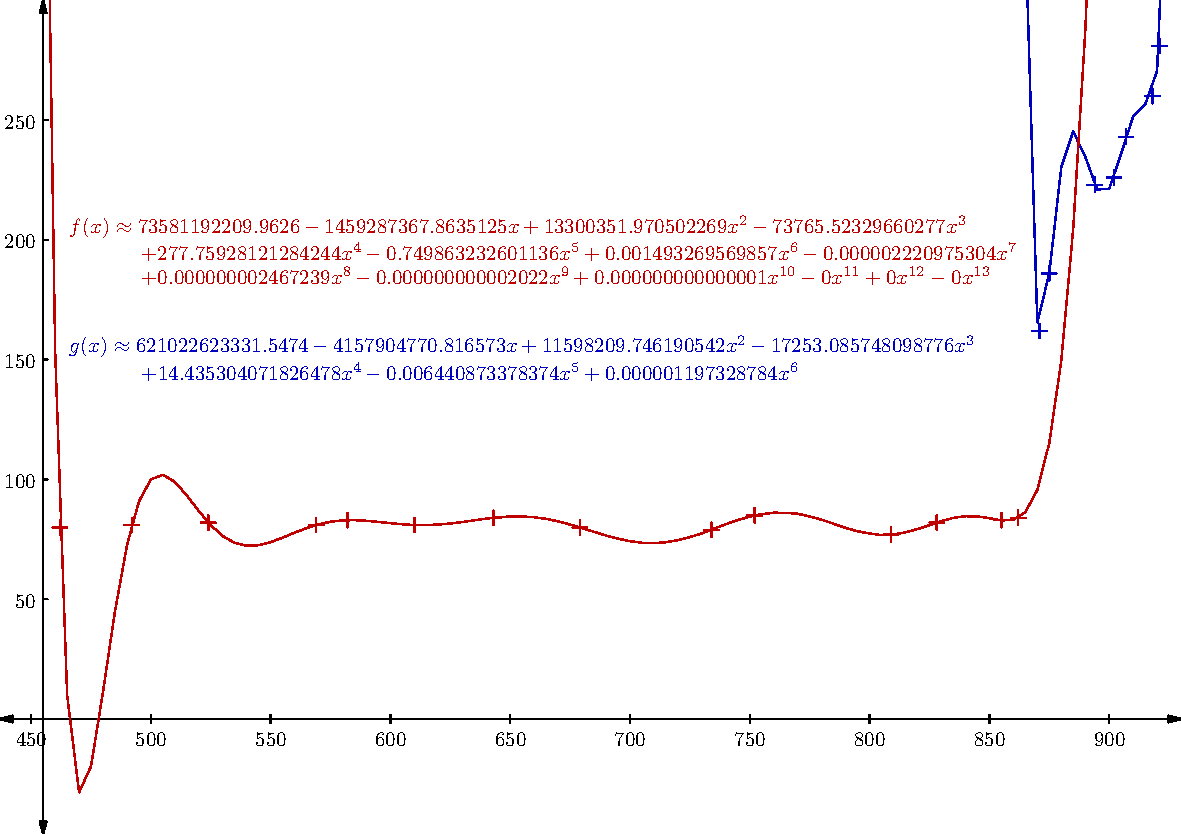
\includegraphics[scale=0.85]{graphiques/pdf_output/inter_tp2_ex3.pdf}
	\caption{Interpolation de Newton et Neuville -- (Tableaux \ref{inter_tp2_ex3_depenses_bas} \& \ref{inter_tp2_ex3_depenses_haut})}
      \end{figure}
    \newpage
    \section{Comparaison}
  \chapter{Approximation}
    \section{Régression linéaire}
      \subsection{Présentation}
      \subsection{Programme}
	\lstinputlisting[style=customc]{reglin.c}
    \section{Ajustement exponentiel}
    
    \section{Ajustement de type ``puissance"}
    \newpage
    \section{Résultats de tests}
      \subsection{Exemple tiré d'un TD}
	\begin{table}[h]
	  \centering
	  \begin{tabular}{| c | c | c | c | c | c |}
	    \hline 
	    $x_{i}$ & $0.5$ & $1$ & $1.5$ & $2$ & $2.5$ \\ 
	    \hline 
	    $y_{i}$ & $0.49$ & $1.6$ & $3.36$ & $6.44$ & $10.16$ \\ 
	    \hline 
	  \end{tabular}
	  \caption{Série 1}
	  \label{approx_td3_ex6}
	\end{table}
	\begin{figure}[h]
	  \centering
	  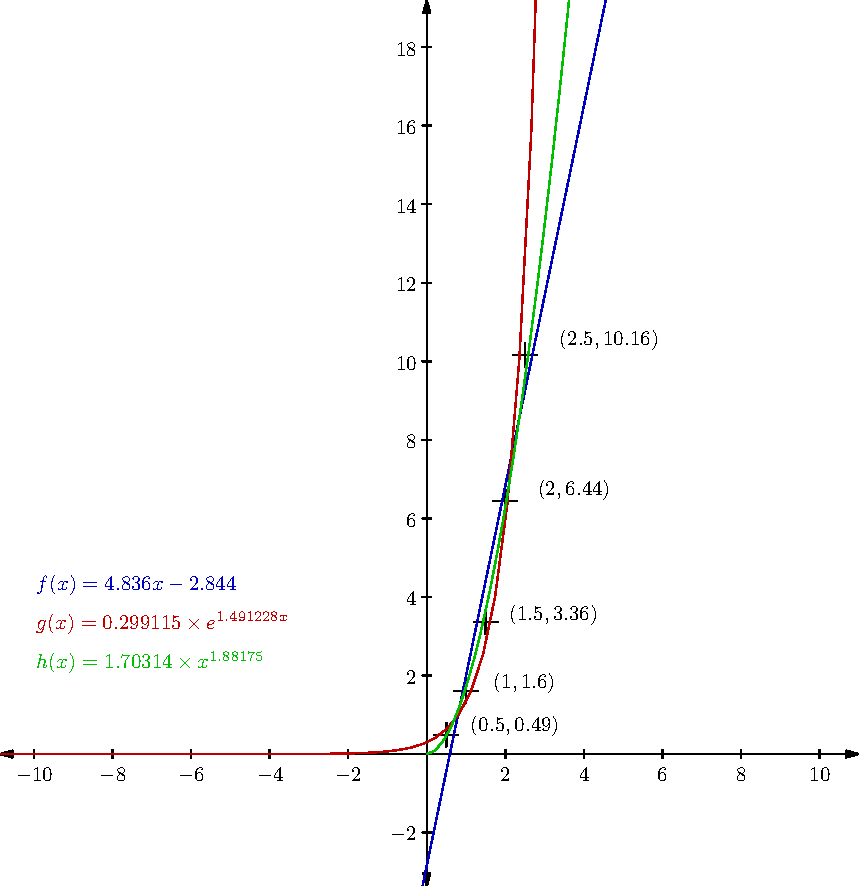
\includegraphics{graphiques/pdf_output/reglin.pdf}
	  \caption{Régression linéaire -- (Tableau \ref{approx_td3_ex6})}
	\end{figure}
      \newpage
      \subsection{Série d'Anscombe}
	\begin{table}[h]
	  \centering
	  \begin{tabular}{| c | c | c | c | c | c | c | c | c | c | c | c |}
	    \hline 
	    $x_{i}$ & $10$ & $8$ & $13$ & $9$ & $11$ & $14$ & $6$ & $4$ & $12$ & $7$ & $5$ \\ 
	    \hline 
	    $y^{(A)}_{i}$ & $8.04$ & $6.95$ & $7.58$ & $8.81$ & $8.33$ & $9.96$ & $7.24$ & $4.26$ & $10.84$ & $4.82$ & $5.68$ \\ 
	    \hline 
	  \end{tabular}
	  \caption{Série dûe à Anscombe}
	  \label{approx_tp2_ex1}
	\end{table}
	\begin{figure}[h]
	  \centering
	  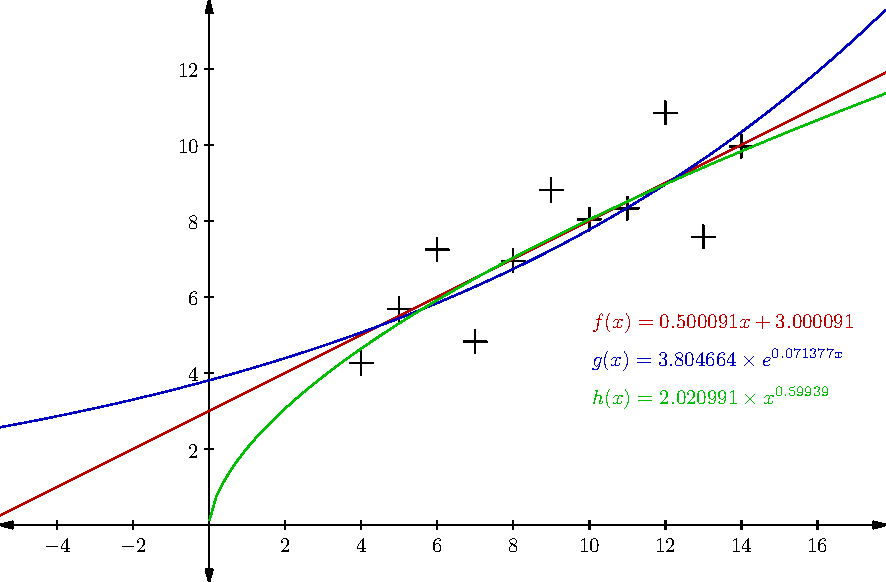
\includegraphics{graphiques/pdf_output/reglin_tp2_ex1.pdf}
	  \caption{Régression linéaire -- (Tableau \ref{approx_tp2_ex1})}
	\end{figure}
	\newpage
      \subsection{3 séries}
	\begin{table}[h]
	  \centering
	  \begin{tabular}{| c | c | c | c | c | c | c | c | c | c | c | c |}
	    \hline 
	    $x_{i}$ & $10$ & $8$ & $13$ & $9$ & $11$ & $14$ & $6$ & $4$ & $12$ & $7$ & $5$ \\ 
	    \hline 
	    $y^{(1)}_{i}$ & $9.14$ & $8.14$ & $8.74$ & $8.77$ & $9.26$ & $8.10$ & $6.13$ & $3.10$ & $9.13$ & $7.26$ & $4.74$ \\ %s1
	    \hline 
	    $y^{(2)}_{i}$ & $7.46$ & $6.77$ & $12.74$ & $7.11$ & $7.81$ & $8.84$ & $6.08$ & $5.39$ & $8.15$ & $6.42$ & $5.73$ \\ %s2
	    \hline 
	    $y^{(3)}_{i}$ & $6.58$ & $5.76$ & $7.71$ & $8.84$ & $8.47$ & $7.04$ & $5.25$ & $12.50$ & $5.56$ & $7.91$ & $6.89$ \\ %s3
	    \hline 
	    $y^{(A)}_{i}$ & $8.04$ & $6.95$ & $7.58$ & $8.81$ & $8.33$ & $9.96$ & $7.24$ & $4.26$ & $10.84$ & $4.82$ & $5.68$ \\ %anscombe
	    \hline 
	  \end{tabular}
	  \caption{3 séries $S^{(1)}$, $S^{(2)}$ et $S^{(3)}$ comparées à Anscombe}
	  \label{approx_tp2_ex2}
	\end{table}
	Série (1) :
	\newline
	Regression linéaire par une droite : $P(x) = 3.000909 + 0.500000 \cdot x$
	\newline
	Erreur moyenne : $0.967934$
	\newline
	\newline
	Série (2) :
	\newline
	Regression linéaire par une droite : $P(x) = 3.002455 + 0.499727 \cdot x$
	\newline
	Erreur moyenne : $0.715967$
	
	\begin{figure}[h]
	  \centering
	  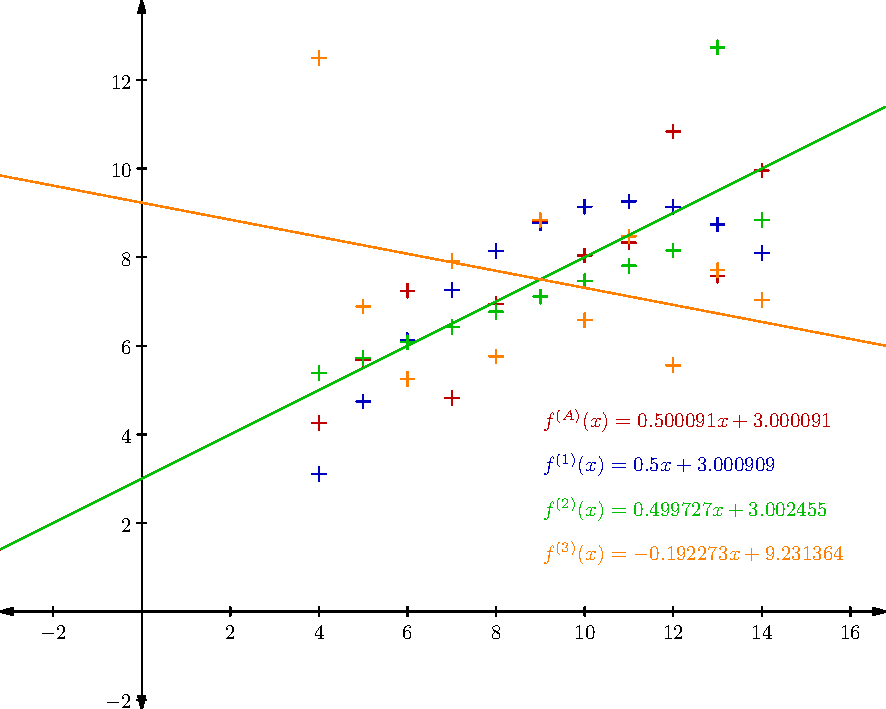
\includegraphics{graphiques/pdf_output/reglin_tp2_ex2_1.pdf}
	  \caption{Régression linéaire -- (Tableau \ref{approx_tp2_ex2})}
	\end{figure}
	\newpage
        Regression linéaire par une exponentielle :$P(x) = 3.417548 \cdot \exp(0.082249 \cdot x)$
        
        Erreur moyenne : $1.187786$

        Regression linéaire par une exponentielle :$P(x) = 4.100273 \cdot \exp(0.063981 \cdot x)$
        
        Erreur moyenne : $0.590601$

	\begin{figure}[h]
	  \centering
	  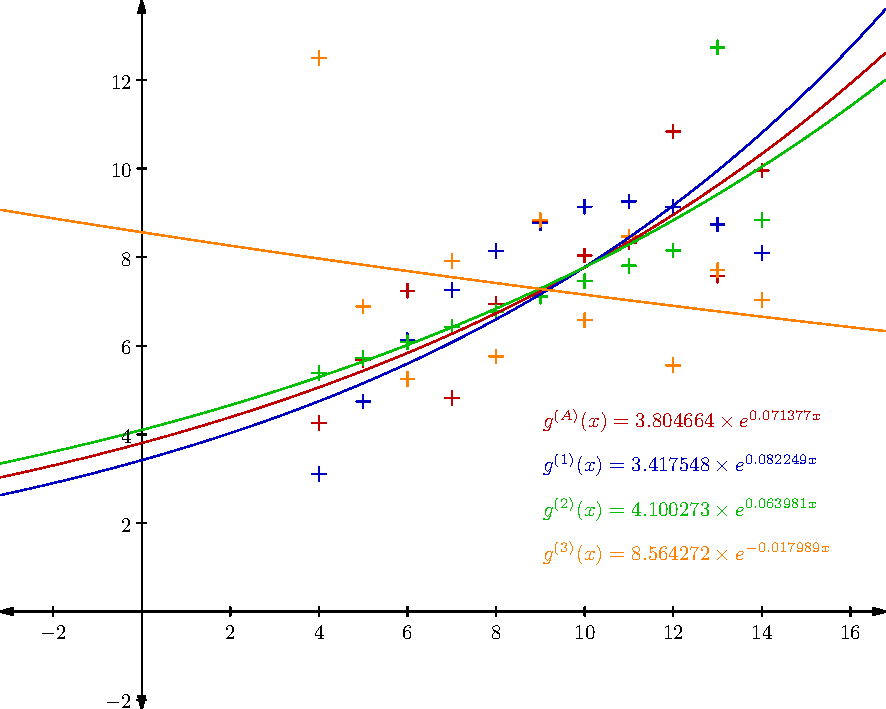
\includegraphics{graphiques/pdf_output/reglin_tp2_ex2_2.pdf}
	  \caption{Approximation par ajustement exponentiel -- (Tableau \ref{approx_tp2_ex2})}
	\end{figure}
	\newpage
        Regression linéaire par une puissance : $P(x) = 1.453451 \cdot x^{0.749910}$
        
        Erreur moyenne : $0.950634$

        Regression linéaire par une puissance :$P(x) = 2.478570 \cdot x^{0.507328}$
        
        Erreur moyenne : $0.682932$
	\begin{figure}[h]
	  \centering
	  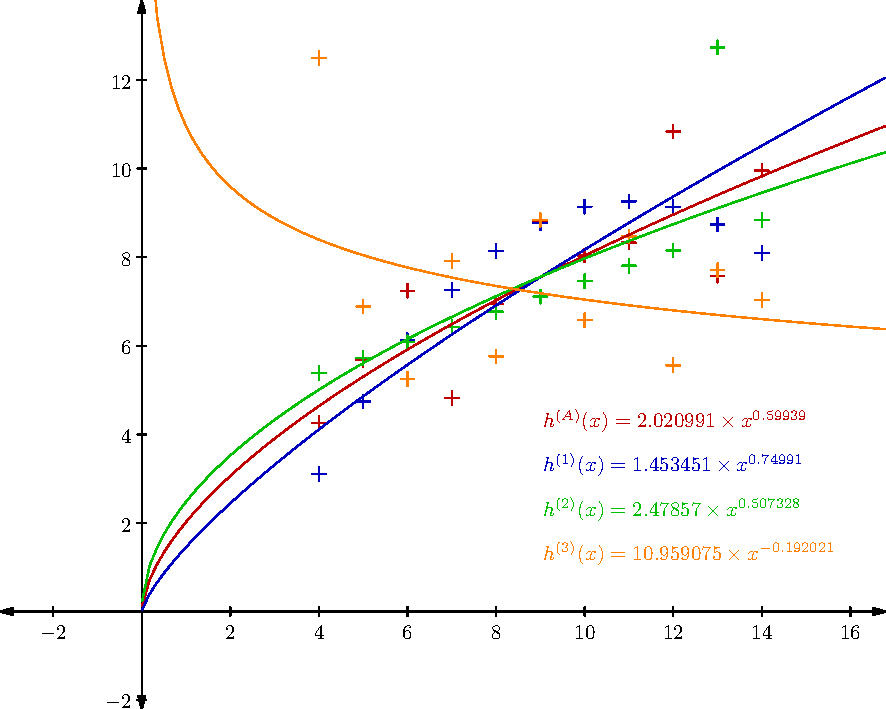
\includegraphics{graphiques/pdf_output/reglin_tp2_ex2_3.pdf}
	  \caption{Approximation par ajustement ``puissance" -- (Tableau \ref{approx_tp2_ex2})}
	\end{figure}
      \newpage
      \subsection{Dépenses mensuelles et revenus}
	\begin{table}[h]
	  \centering
	  \begin{tabular}{| c | c | c | c | c | c | c | c | c | c | c | c |}
	    \hline 
	    $x_{i}$ (R) & $752$ & $855$ & $871$ & $734$ & $610$ & $582$ & $921$ & $492$ & $569$ & $462$ & $907 $ \\ 
	    \hline 
	    $y_{i}$ (D) & $85$ & $83$ & $162$ & $79$ & $81$ & $83$ & $281$ & $81$ & $81$ & $80$ & $243 $ \\ 
	    \hline 
	  \end{tabular}
	  \caption{Série 1}
	  \label{approx_tp2_ex3_1}
	\end{table}
	\begin{table}[h]
	  \centering
	  \begin{tabular}{| c | c | c | c | c | c | c | c | c | c | c |}
	  \hline 
	  $x_{i}$ (R) & $643$ & $862$ & $524$ & $679$ & $902$ & $918$ & $828$ & $875$ & $809$ & $894$ \\ 
	  \hline 
	  $y_{i}$ (D) & $84$ & $84$ & $82$ & $80$ & $226$ & $260$ & $82$ & $186$ & $77$ & $223$ \\ 
	  \hline 
	  \end{tabular}
	  \caption{Série 2}
	  \label{approx_tp2_ex3_2}
	\end{table}
	Série 1 :
	\newline
	Regression linéaire par une droite :$ P(x) =  - 98.368005 + 0.312192 \cdot x$
	\newline
	Erreur moyenne : $38.488186$
	\newline
	\newline
	Regression linéaire par une exponentielle :$P(x) = 24.011644 \cdot \exp(0.002124 \cdot x)$
	\newline
	Erreur moyenne : $33.486916$
	\newline
	\newline
	Regression linéaire par une puissance :$P(x) = 0.015258 \cdot x^{1.356482}$
	\newline
	Erreur moyenne : $36.660388$
	\newline 
	\newline
	\newline
	Série 2 :
	\newline
	Regression linéaire par une droite :$P(x) =  - 164.266162 + 0.381480 \cdot x$
	\newline
	Erreur moyenne : $46.455702$
	\newline
	\newline
	Regression linéaire par une exponentielle :$P(x) = 14.780629 \cdot \exp(0.002657 \cdot x)$
	\newline
	Erreur moyenne : $45.099159$
	\newline
	\newline
	Regression linéaire par une puissance :$P(x) = 0.000785  \cdot x^{1.793989}$
	\newline
	Erreur moyenne : $47.682118$
  %       \begin{figure}[h]
  % 	\centering
  % 	\includegraphics[scale=0.7]{}
  % 	\caption{Approximation -- (Tableau \ref{Jeux d'essais approximation 3.3 Série 1})}
  %       \end{figure}
      \newpage
      
      \subsection{Série chronologique avec accroissement exponentiel}
      
	\begin{table}[h]
	  \centering
	  \begin{tabular}{| c | c | c | c | c | c | c | c | c | c | c |}
	    \hline 
	    $x_{i}$ & $88$ & $89$ & $90$ & $91$ & $92$ & $93$ & $94$ & $95$ & $96$ & $97$ \\ 
	    \hline 
	    $y_{i}$ & $5.89$ & $6.77$ & $7.97$ & $9.11$ & $10.56$ & $12.27$ & $13.92$ & $15.72$ & $17.91$ & $22.13$ \\ 
	    \hline 
	  \end{tabular}
	  \caption{Série}
	  \label{approx_tp2_ex4}
	\end{table}
      \newpage
      
      \subsection{Vérification de la loi de Pareto}
	\begin{table}[h]
	  \centering
	  \begin{tabular}{| c | c | c | c | c | c | c | c |}
	      \hline 
	      $x_{i}$ & $20$ & $30$ & $40$ & $50$ & $100$ & $300$ & $500$ \\ 
	      \hline 
	      $y_{i}$ & $352$ & $128$ & $62.3$ & $35.7$ & $6.3$ & $0.4$ & $0.1$ \\ 
	      \hline 
	  \end{tabular}
	  \caption{Relation entre revenu et nombre de personnes ayant un revenu supérieur}
	  \label{approx_tp2_ex5}
	\end{table}
  \chapter{Conclusion}

\end{document}


      
%       \newpage      
%       \begin{table}[h]
% 	\centering
% 		\begin{tabular}{| c | c | c | c | c | c | c | c | c | c | c | c | c | c | c | c | c | c | c | c | c |}
% 	\hline 
% 	$x_{i}$ & $0$ & $2$ & $4$ & $6$ & $8$ & $10$ & $12$ & $14$ & $16$ & $18$ & $20$ & $22$ & $24$ & $26$ & $28$ & $30$ & $32$ & $34$ & $36$ & $38$ \\ 
% 	\hline 
% 	$y_{i}$ & $0.999870$ & $0.999970$ & $1$ & $0.999970$ & $0.999880$ & $0.999730$ & $0.999530$ & $0.999530$ & $0.998970$ & $0.998460$ & $0.998050$ & $0.999751$ & $0.997050$ & $0.996500$ & $0.996640$ & $0.995330$ & $0.994720$ & $0.994720$ & $0.993330$ & $0.993260$ \\ 
% 	\hline 
% 	\end{tabular}
% 	\caption{3.1 Densité de l'eau en fonction de la température}
% 	%\label{Jeux d'essais approximation 3.0}
% 		\end{table}
% 	
% 	Regression linéaire par une droite : $P(x) = 1.001302 - 0.000186 \cdot x$
% 	
% 	Erreur moyenne : $0.000665$
% 	
% 	Regression linéaire par une exponentielle : $P(x) = 1.001308 \cdot \exp(-0.000187 \cdot x) $
% 	
% 	Erreur moyenne : $0.000667$
% 	
% 	Regression linéaire par une puissance : Pas de résultat, lors du changement de variable, on calcule $\log_{2}(0)$ qui n'est pas défini.
	
	% 		\begin{figure}[h]
% 	\centering
% 	\includegraphics[scale=0.7]{graphiques/pdf_output/}
% 	\caption{Approximation -- (Tableau \ref{Jeux d'essais approximation 3.0})}
%       \end{figure}
%       \newpage
      
%       \begin{figure}[h]
% 	\centering
% 	\includegraphics[scale=0.7]{}
% 	\caption{Approximation-- (Tableau \ref{Jeux d'essais approximation 3.3 Série 2})}
%       \end{figure}


%       \newpage
%       \begin{table}[h]
% 	\centering
% 	\begin{tabular}{| c | c | c | c | c | c | c | c | c | c | c | c | c | c | c | c | c | c | c | c | c | c |}
% 	  \hline 
% 	  $x_{i}$ & $752$ & $855$ & $871$ & $734$ & $610$ & $582$ & $921$ & $492$ & $569$ & $462$ & $907$ & $643$ & $862$ & $524$ & $679$ & $902$ & $918$ & $828$ & $875$ & $809$ & $894$ \\ 
% 	  \hline 
% 	  $y_{i}$ & $85$ & $83$ & $162$ & $79$ & $81$ & $83$ & $281$ & $81$ & $81$ & $80$ & $243$ & $84$ & $84$ & $82$ & $80$ & $226$ & $260$ & $82$ & $186$ & $77$ & $223$ \\ 
% 	  \hline 
% 	\end{tabular}
% 	\caption{Série1-2 dépense}
% 	%\label{Jeux d'essais interpolation 3.3 Série 1 et 2}
%       \end{table}
% 	Regression linéaire par une droite :$P(x) =  - 112.658491 + 0.324356 \cdot x$
% 	
% 	Erreur moyenne : $43.378231$
% 	
% 	Reression linéaire par une exponentielle :$P(x) = 21.399929\cdot \exp(0.002238 \cdot x)$
% 	
% 	Erreur moyenne : $40.094599$
% 	
% 	Regression linéaire par une puissance :$P(x) = 0.007872 \cdot x^{1.453059}$
% 	
% 	Erreur moyenne : $42.696155$
%       
%       \begin{figure}[h]
% 	\centering
% 	\includegraphics[scale=0.7]{}
% 	\caption{Approximation -- (Tableau \ref{Jeux d'essais interpolation 3.3 Série 1 et 2})}
%       \end{figure}
